\chapter{Mesure de temps}
\label{an:MesTemps}

Cette annexe vient présenter les captures d'écrant de l'oscilloscope.

\section{Avec la communication en UART}
\subsection{Mesure avec les 4 inducteurs}

\begin{figure}[H]
    \centering
    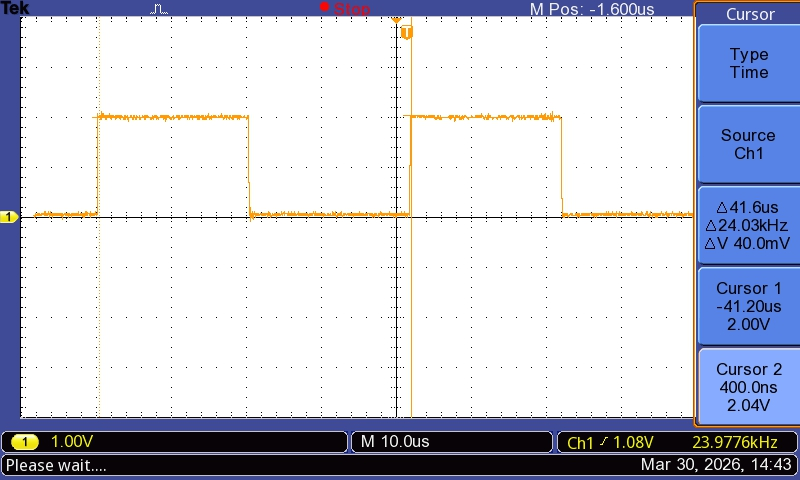
\includegraphics[width=1\linewidth]{assets/appendix/05-MesureTemps/AvecUART/4-Inducteurs/Periode.JPG}
    \caption{Mesure de la période}
\end{figure}

\begin{figure}[H]
    \centering
    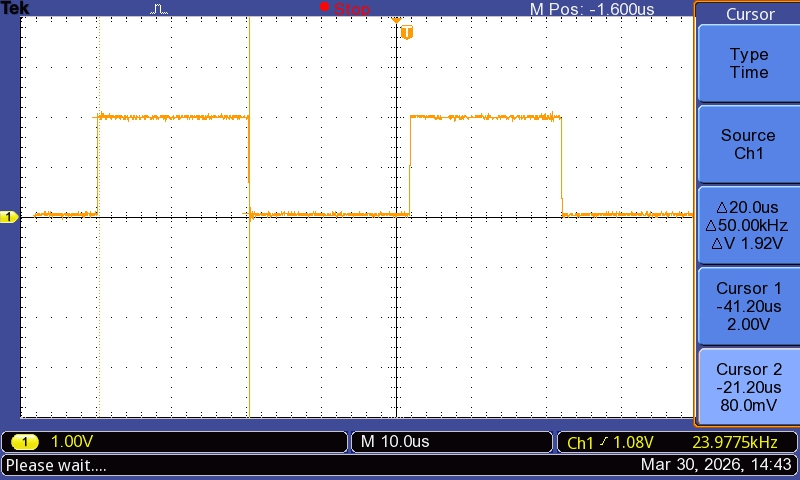
\includegraphics[width=1\linewidth]{assets/appendix/05-MesureTemps/AvecUART/4-Inducteurs/InterruptionTot.JPG}
    \caption{Mesure de l'interruption globale}
\end{figure}

\begin{figure}[H]
    \centering
    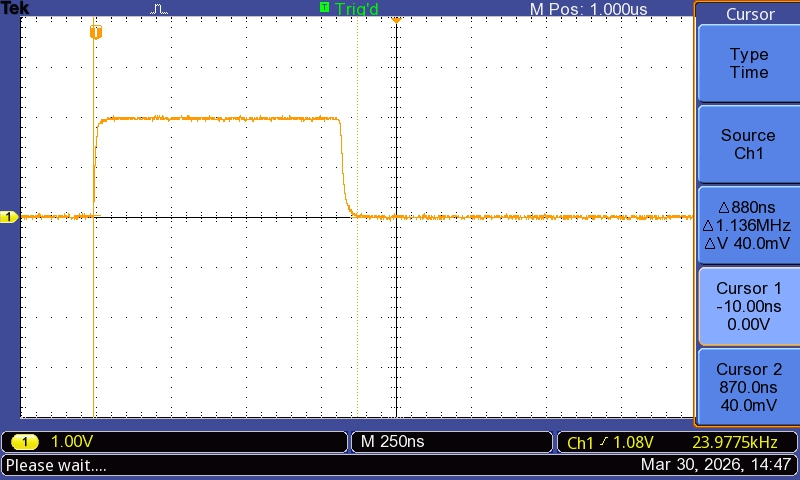
\includegraphics[width=1\linewidth]{assets/appendix/05-MesureTemps/AvecUART/4-Inducteurs/ADC.JPG}
    \caption{Mesure des ADC}
\end{figure}

\begin{figure}[H]
    \centering
    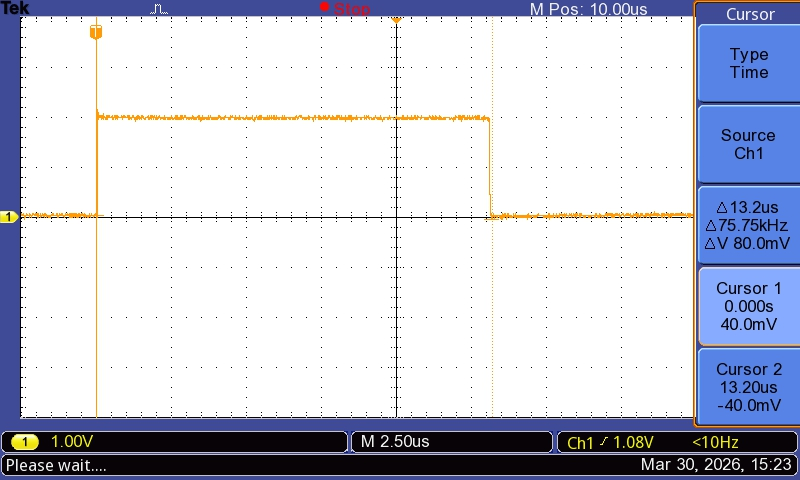
\includegraphics[width=1\linewidth]{assets/appendix/05-MesureTemps/AvecUART/4-Inducteurs/StateMachine.JPG}
    \caption{Mesure de la machine d'état et de la régulation}
\end{figure}

\begin{figure}[H]
    \centering
    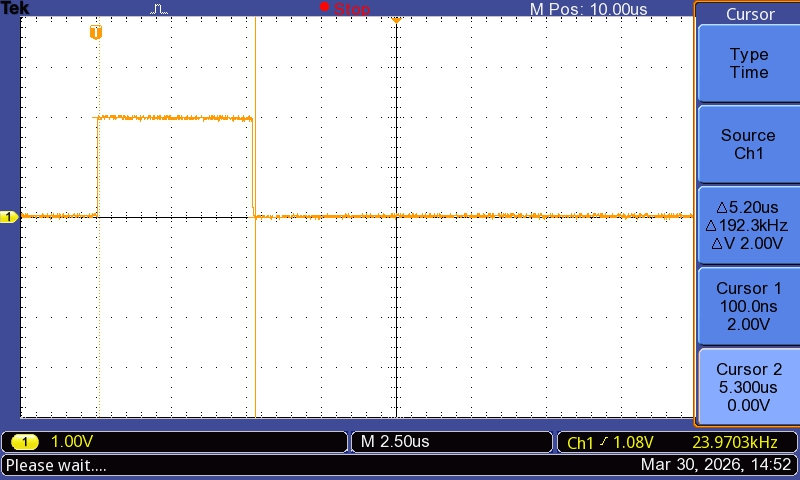
\includegraphics[width=1\linewidth]{assets/appendix/05-MesureTemps/AvecUART/4-Inducteurs/PWM.JPG}
    \caption{Mesure des signaux PWM}
\end{figure}

\subsection{Mesure avec les inducteurs 1 et 2}

\begin{figure}[H]
    \centering
    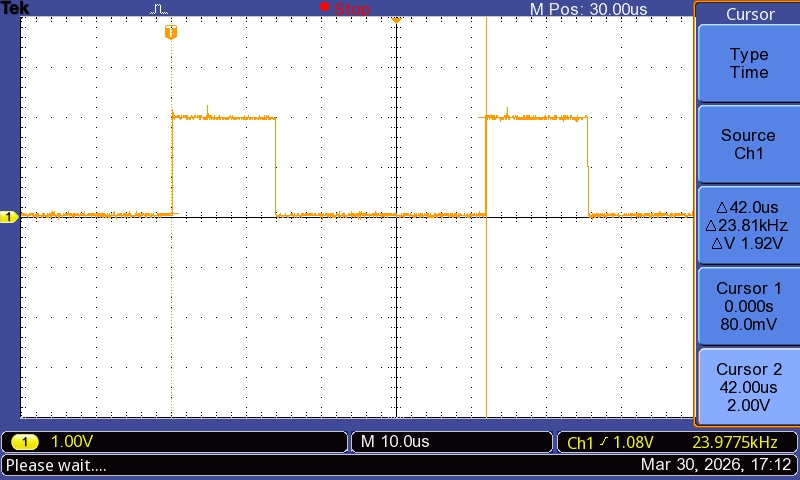
\includegraphics[width=1\linewidth]{assets/appendix/05-MesureTemps/AvecUART/Inducteurs-1-2/Periode.JPG}
    \caption{Mesure de la période}
\end{figure}

\begin{figure}[H]
    \centering
    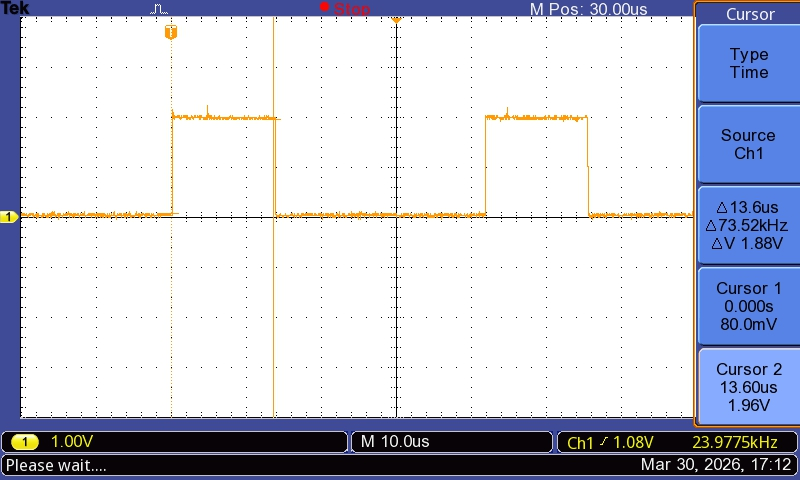
\includegraphics[width=1\linewidth]{assets/appendix/05-MesureTemps/AvecUART/Inducteurs-1-2/InteruptTot.JPG}
    \caption{Mesure de l'interruption globale}
\end{figure}

\begin{figure}[H]
    \centering
    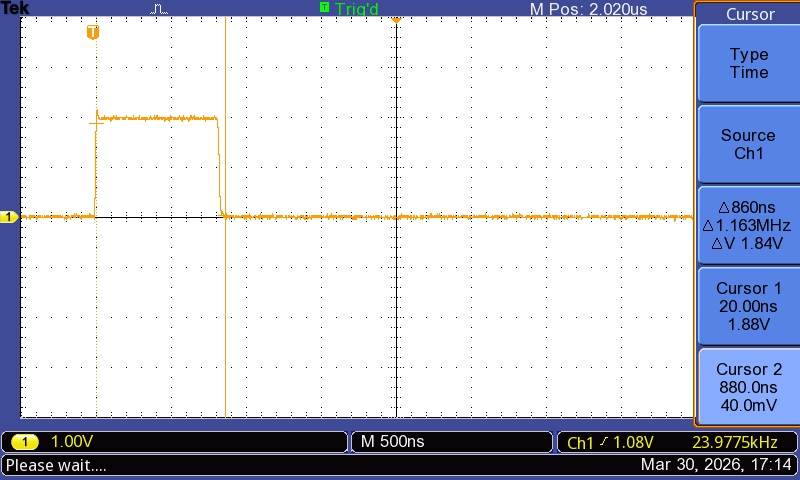
\includegraphics[width=1\linewidth]{assets/appendix/05-MesureTemps/AvecUART/Inducteurs-1-2/ADC.JPG}
    \caption{Mesure des ADC}
\end{figure}

\begin{figure}[H]
    \centering
    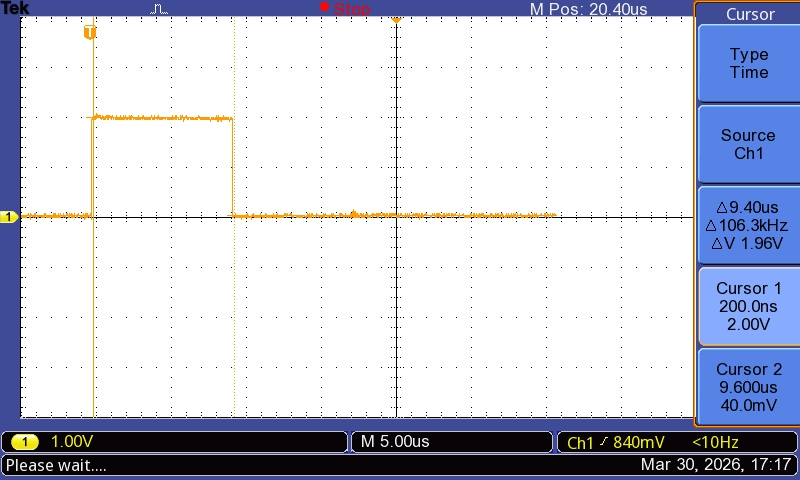
\includegraphics[width=1\linewidth]{assets/appendix/05-MesureTemps/AvecUART/Inducteurs-1-2/StateMachine.JPG}
    \caption{Mesure de la machine d'état et de la régulation}
\end{figure}

\begin{figure}[H]
    \centering
    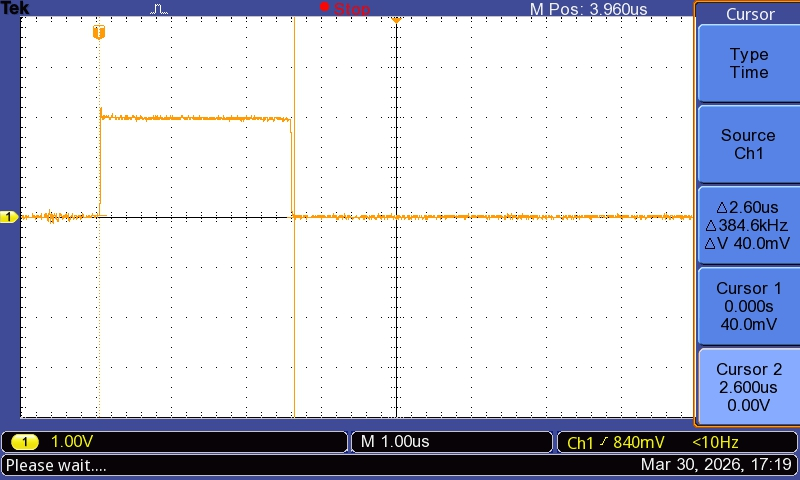
\includegraphics[width=1\linewidth]{assets/appendix/05-MesureTemps/AvecUART/Inducteurs-1-2/PWM.JPG}
    \caption{Mesure des signaux PWM}
\end{figure}

\subsection{Mesure avec les inducteurs 3 et 4}

\begin{figure}[H]
    \centering
    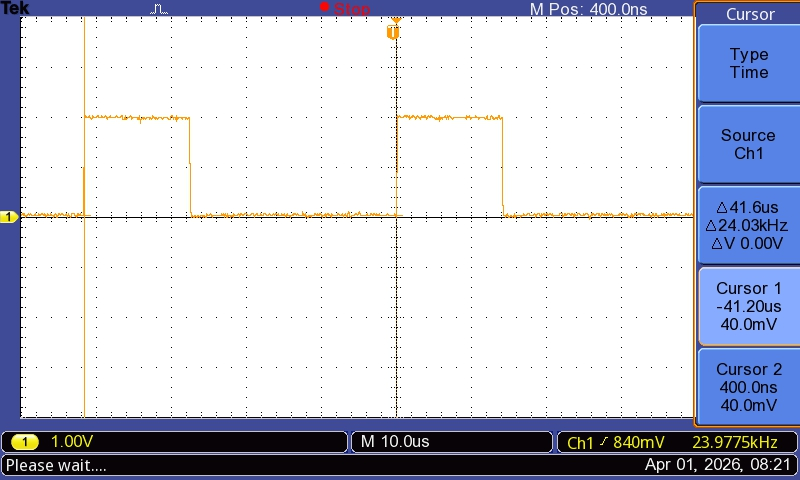
\includegraphics[width=1\linewidth]{assets/appendix/05-MesureTemps/AvecUART/Inducteurs-3-4/Periode.JPG}
    \caption{Mesure de la période}
\end{figure}

\begin{figure}[H]
    \centering
    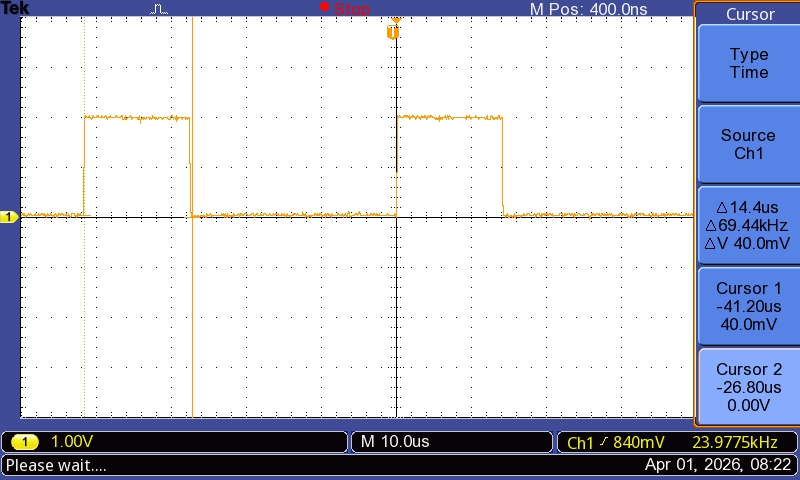
\includegraphics[width=1\linewidth]{assets/appendix/05-MesureTemps/AvecUART/Inducteurs-3-4/InteruptTot.JPG}
    \caption{Mesure de l'interruption globale}
\end{figure}

\begin{figure}[H]
    \centering
    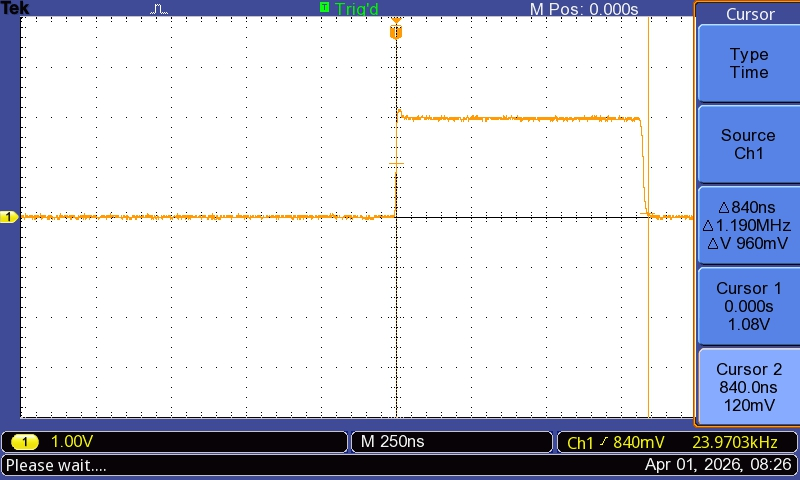
\includegraphics[width=1\linewidth]{assets/appendix/05-MesureTemps/AvecUART/Inducteurs-3-4/ADC.JPG}
    \caption{Mesure des ADC}
\end{figure}

\begin{figure}[H]
    \centering
    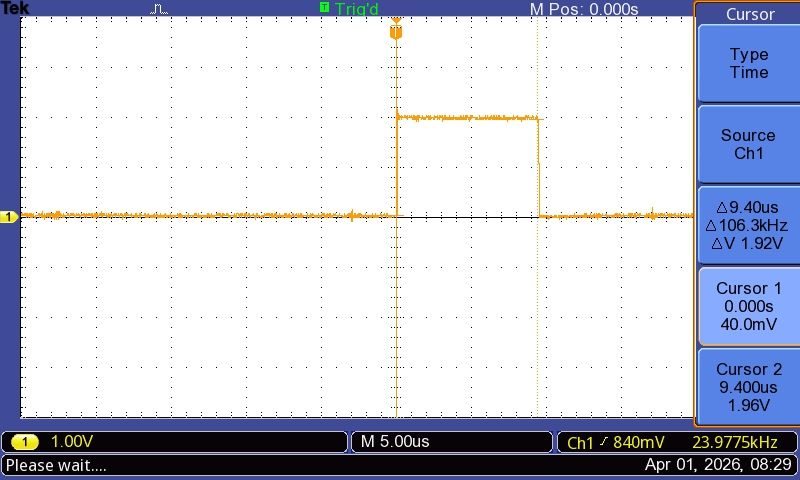
\includegraphics[width=1\linewidth]{assets/appendix/05-MesureTemps/AvecUART/Inducteurs-3-4/StateMachine.JPG}
    \caption{Mesure de la machine d'état et de la régulation}
\end{figure}

\begin{figure}[H]
    \centering
    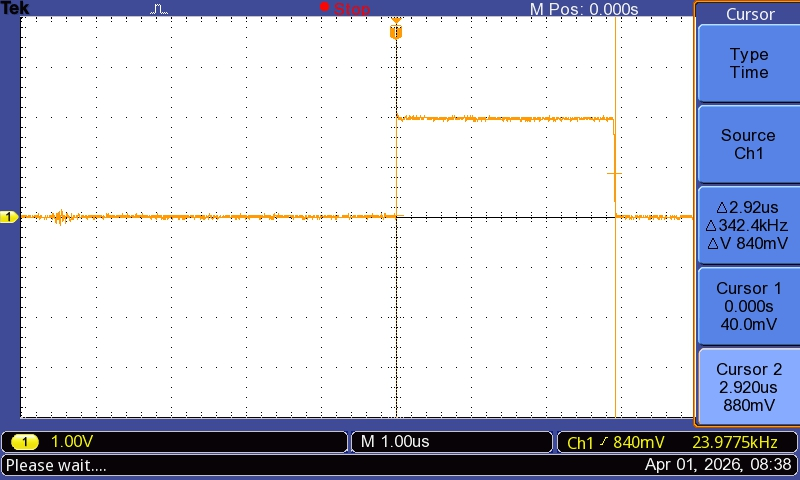
\includegraphics[width=1\linewidth]{assets/appendix/05-MesureTemps/AvecUART/Inducteurs-3-4/PWM.JPG}
    \caption{Mesure des signaux PWM}
\end{figure}


\section{Sans la communication en UART}
\subsection{Mesure avec les 4 inducteurs}

\begin{figure}[H]
    \centering
    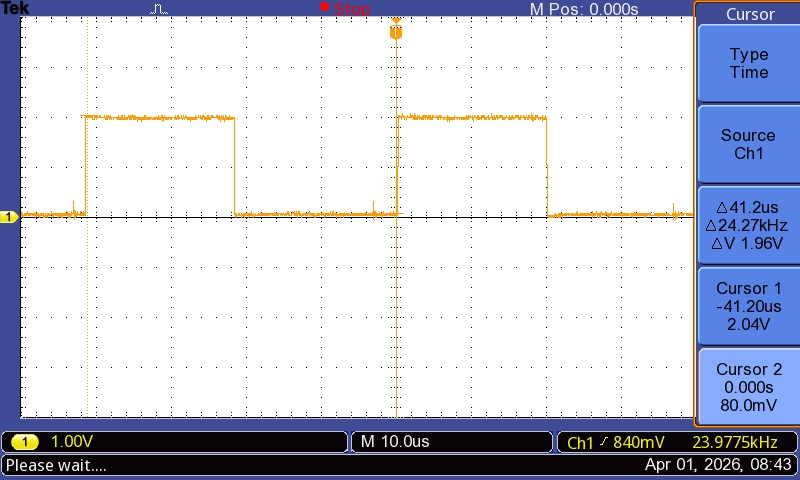
\includegraphics[width=1\linewidth]{assets/appendix/05-MesureTemps/SansUART/4-Inducteurs/TEK0000.JPG}
    \caption{Mesure de la période}
\end{figure}

\begin{figure}[H]
    \centering
    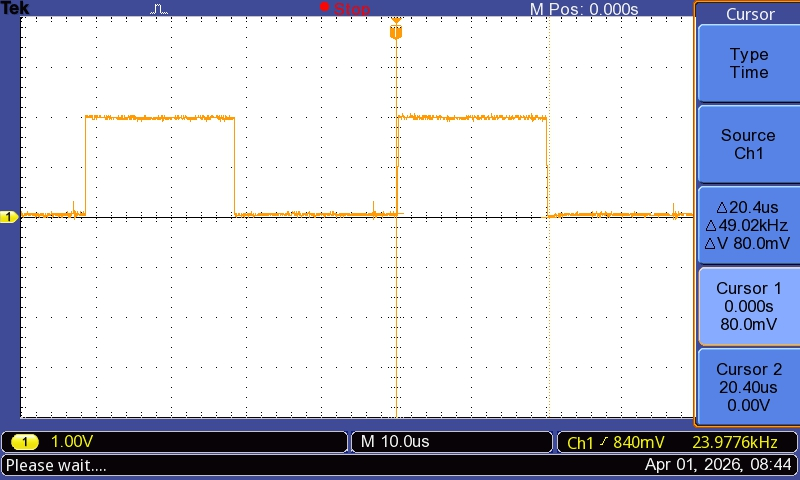
\includegraphics[width=1\linewidth]{assets/appendix/05-MesureTemps/SansUART/4-Inducteurs/TEK0001.JPG}
    \caption{Mesure de l'interruption globale}
\end{figure}

\begin{figure}[H]
    \centering
    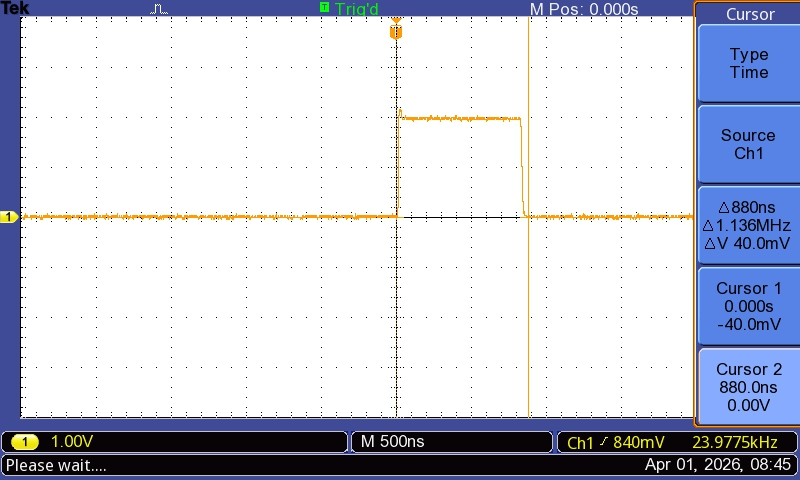
\includegraphics[width=1\linewidth]{assets/appendix/05-MesureTemps/SansUART/4-Inducteurs/TEK0002.JPG}
    \caption{Mesure des ADC}
\end{figure}

\begin{figure}[H]
    \centering
    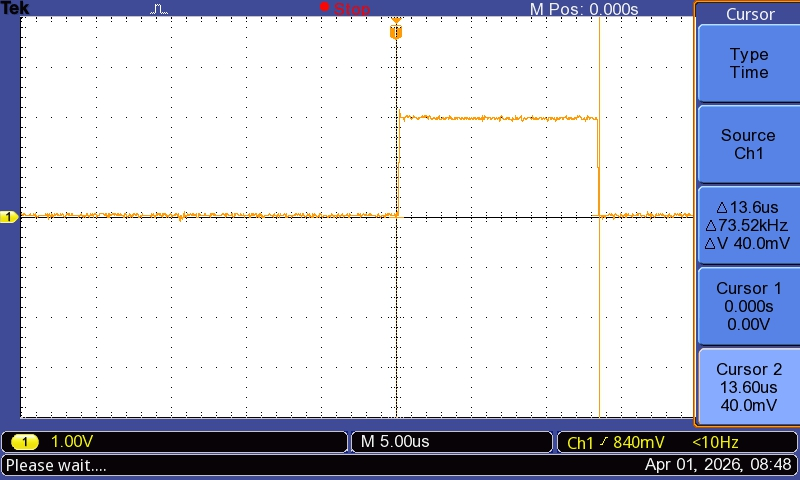
\includegraphics[width=1\linewidth]{assets/appendix/05-MesureTemps/SansUART/4-Inducteurs/TEK0003.JPG}
    \caption{Mesure de la machine d'état et de la régulation}
\end{figure}

\begin{figure}[H]
    \centering
    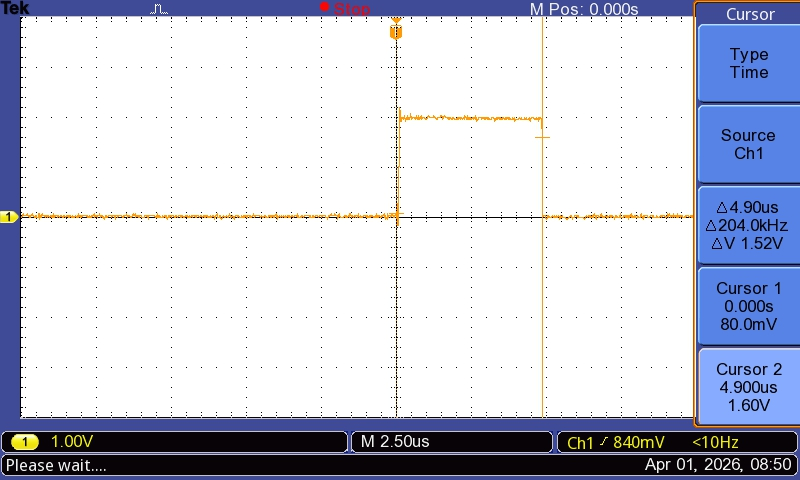
\includegraphics[width=1\linewidth]{assets/appendix/05-MesureTemps/SansUART/4-Inducteurs/TEK0004.JPG}
    \caption{Mesure des signaux PWM}
\end{figure}

\subsection{Mesure avec les inducteurs 1 et 2}

\begin{figure}[H]
    \centering
    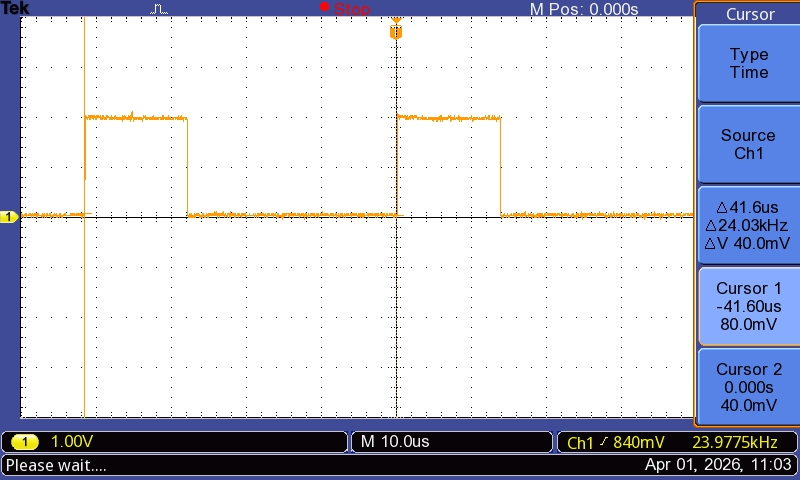
\includegraphics[width=1\linewidth]{assets/appendix/05-MesureTemps/SansUART/Inducteurs-1-2/Period.JPG}
    \caption{Mesure de la période}
\end{figure}

\begin{figure}[H]
    \centering
    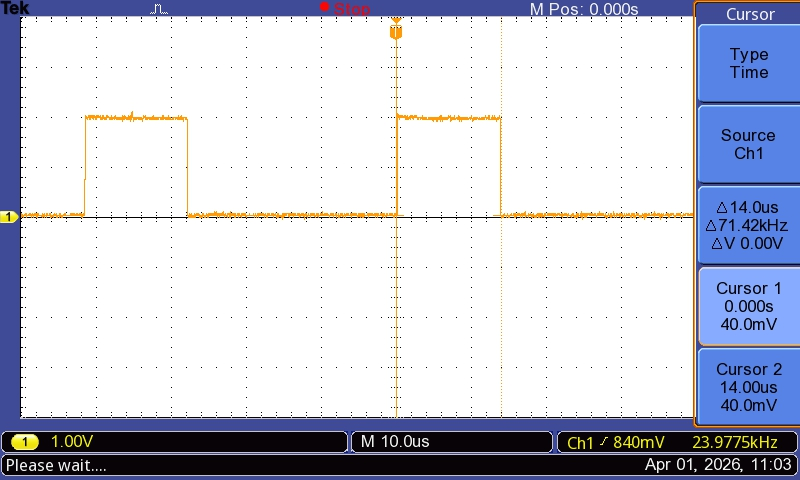
\includegraphics[width=1\linewidth]{assets/appendix/05-MesureTemps/SansUART/Inducteurs-1-2/InteruptTot.JPG}
    \caption{Mesure de l'interruption globale}
\end{figure}

\begin{figure}[H]
    \centering
    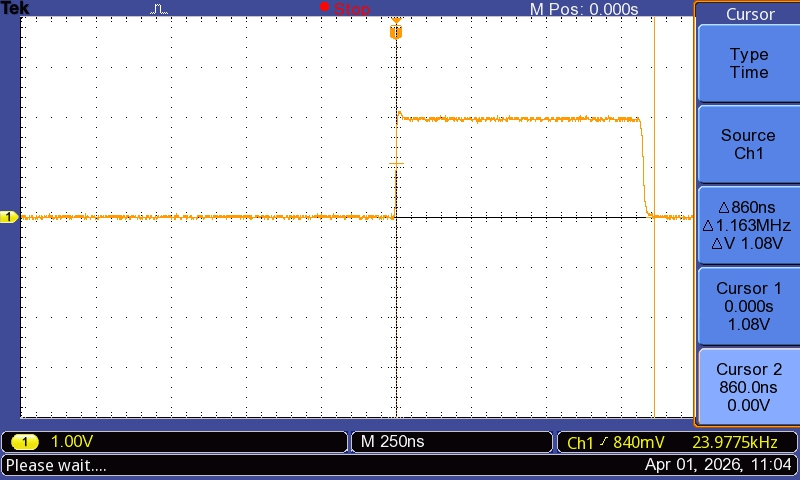
\includegraphics[width=1\linewidth]{assets/appendix/05-MesureTemps/SansUART/Inducteurs-1-2/ADC.JPG}
    \caption{Mesure des ADC}
\end{figure}

\begin{figure}[H]
    \centering
    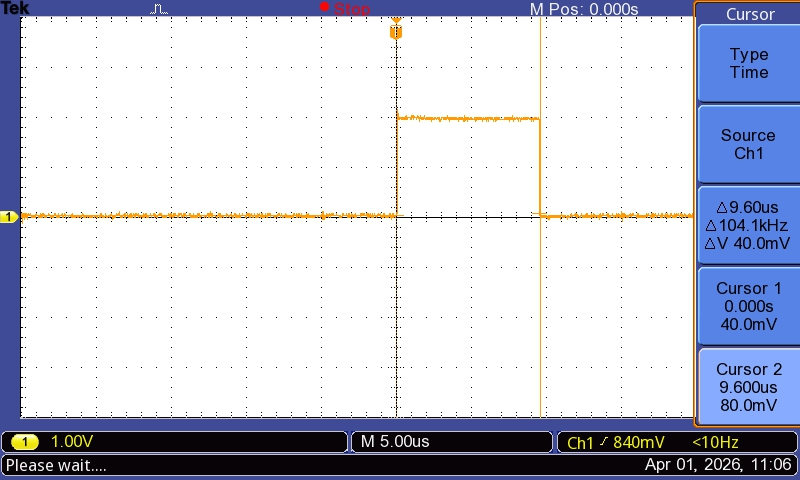
\includegraphics[width=1\linewidth]{assets/appendix/05-MesureTemps/SansUART/Inducteurs-1-2/StateMachine.JPG}
    \caption{Mesure de la machine d'état et de la régulation}
\end{figure}

\begin{figure}[H]
    \centering
    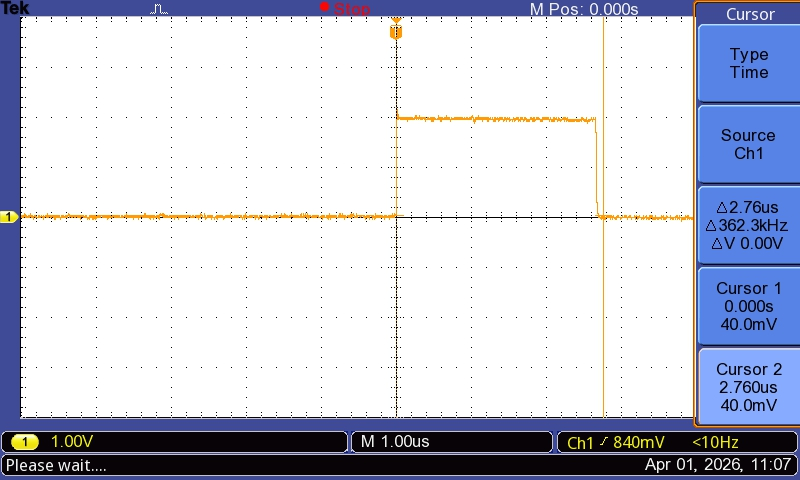
\includegraphics[width=1\linewidth]{assets/appendix/05-MesureTemps/SansUART/Inducteurs-1-2/PWM.JPG}
    \caption{Mesure des signaux PWM}
\end{figure}

\subsection{Mesure avec les inducteurs 3 et 4}

\begin{figure}[H]
    \centering
    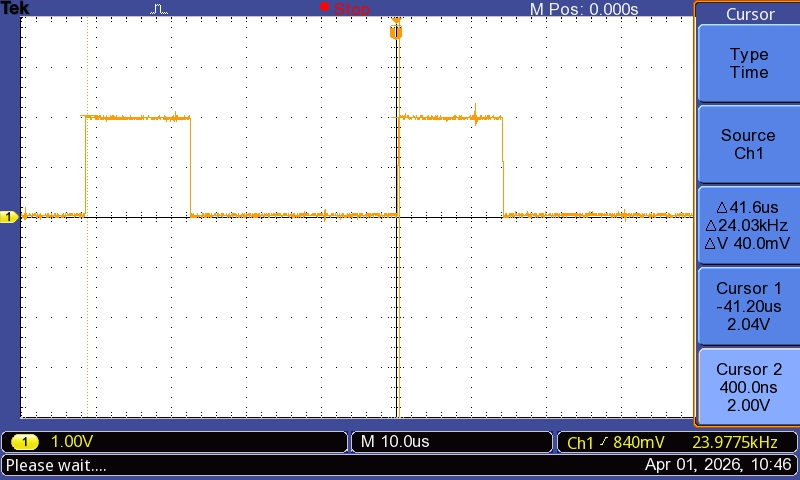
\includegraphics[width=1\linewidth]{assets/appendix/05-MesureTemps/SansUART/Inducteurs-3-4/Periode.JPG}
    \caption{Mesure de la période}
\end{figure}

\begin{figure}[H]
    \centering
    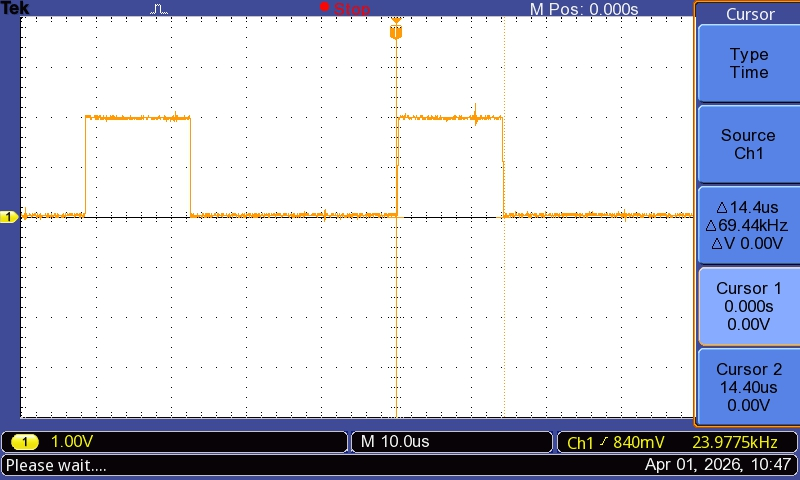
\includegraphics[width=1\linewidth]{assets/appendix/05-MesureTemps/SansUART/Inducteurs-3-4/InteruptTot.JPG}
    \caption{Mesure de l'interruption globale}
\end{figure}

\begin{figure}[H]
    \centering
    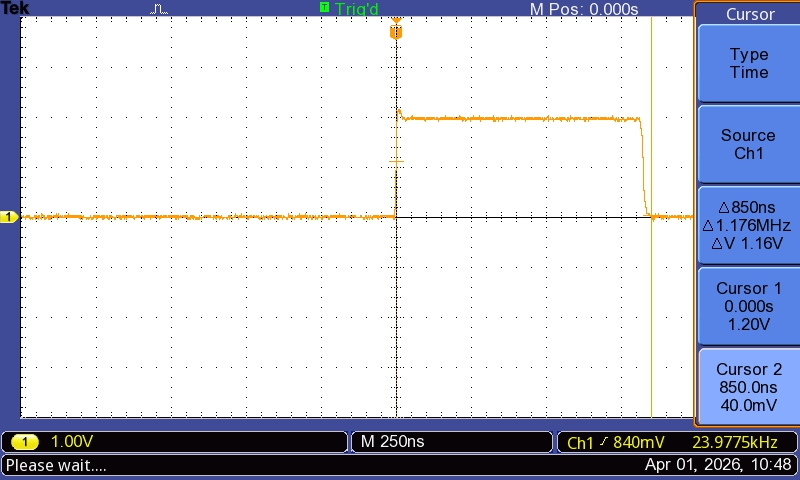
\includegraphics[width=1\linewidth]{assets/appendix/05-MesureTemps/SansUART/Inducteurs-3-4/ADC.JPG}
    \caption{Mesure des ADC}
\end{figure}

\begin{figure}[H]
    \centering
    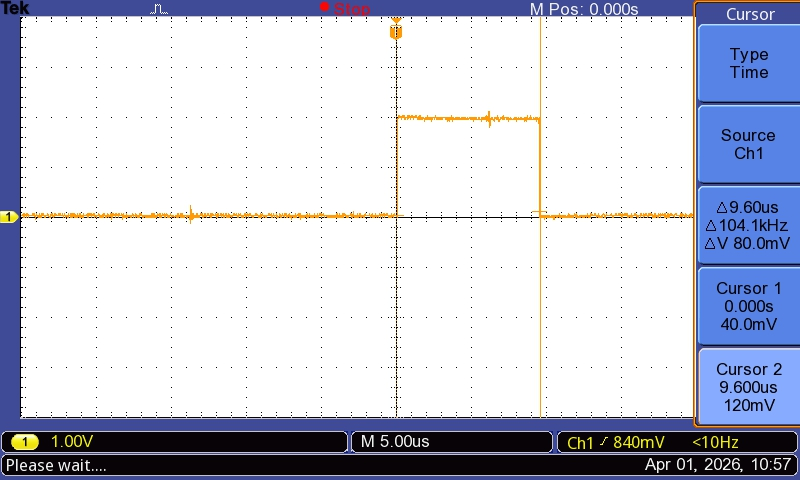
\includegraphics[width=1\linewidth]{assets/appendix/05-MesureTemps/SansUART/Inducteurs-3-4/StateMachine.JPG}
    \caption{Mesure de la machine d'état et de la régulation}
\end{figure}

\begin{figure}[H]
    \centering
    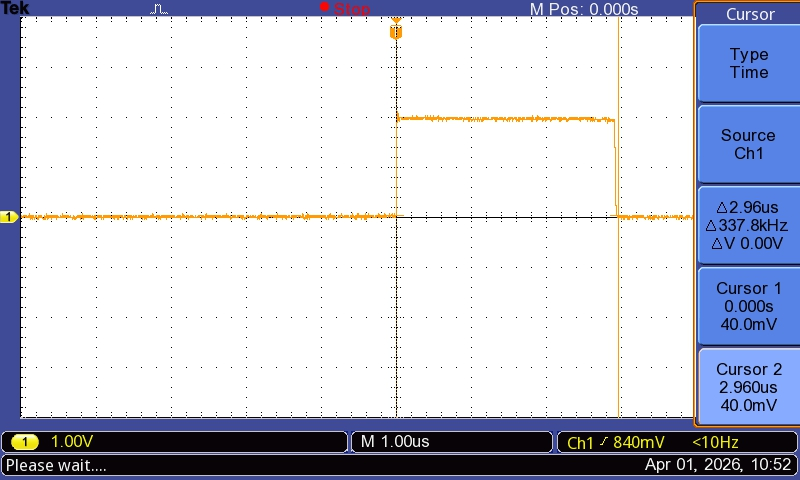
\includegraphics[width=1\linewidth]{assets/appendix/05-MesureTemps/SansUART/Inducteurs-3-4/PWM.JPG}
    \caption{Mesure des signaux PWM}
\end{figure}

\clearpage